\section{\sck}
\label{sec-sck-sck}

\if 0
We (along with my colleague, Cesar A. Stuardo) now present the four \sck
techniques to achieve high colocation factor in one machine (Section
\ref{sc-pil}-\ref{sc-mem}) and summarize how to use these techniques to scale
check the systems (Section \ref{sc-summ}).

The enabler of our methods is the fact that \sck is an offline check, which
provides us the liberty to re-architect distributed systems to be
scale-checkable offline, but without introducing performance overhead online.
%
When $N$ is large, every small optimization in \sck will lead to a multitude of
benefits.
%
When the four techniques are combined, \sck can achieve a colocation factor of
around 500 nodes with high result fidelity.



\subsection{Processing Illusion (PIL)}
\label{sc-pil}

While I/O and memory bottlenecks are often blamed for many scalability problems
\cite{Ousterhout+15-MakingSense,Konstantin+10-HDFSScalability, Wang+14-Exalt},
scalability bugs also could be caused by cascading impacts of CPU-intensive
processing as the example of Cassandra bugs.
%
To emulate CPU-intensive processing, we introduce {\em processing illusion}
(PIL), an approach that {\em replaces an actual processing with \sleep}.  For
example, in the sample Cassandra bug, we can replace the expensive ring-table
update with \ts{sleep(t)} where \ts{t} is an accurate timing of how long the
update takes.


The intuition behind PIL is similar to the intuition behind other
emulation techniques.
%
For example, Exalt provides an illusion of storage space; their insight
was ``how data is processed is  not affected by the content of the data
being written, but only by its size'' \cite{Wang+14-Exalt}.
%
PIL provides an illusion of compute processing; our insight is that
{\em ``the
  key to computation is not the intermediate results, but rather the
  execution time and eventual output''.}
% {\em ``how
%   compute matters is not because of the intermediate computation, but 
% rather by its execution time and output.''}
%

PIL might sound outrageous in the first place, but it is feasible only if 
the following concerns are addressed:
%
% replace compute with sleep
%
How can a function be safely replaced with \sleep \textit{without} changing the
whole processing semantic?  And how to find specific functions that should be
replaced with \sleep?
%
How can we produce the output if the actual compute is skipped?
%
How can we predict the actual compute time (\ts{t}) accurately?

\subsubsection{PIL-Safe Functions}
\label{sc-pil-1}

Our first challenge is to ensure that functions (or code blocks) can be safely
replaced with \sleep, but still retain the cluster-wide behavior and unearth the
bug symptoms.  We name such functions as {\em PIL-safe functions}.
%
We identify two main characteristics of sleep-safe functions:
% by memoization
\begin{enumerate}
\item Memoizable output: a PIL-safe function must have a memoizable
(deterministic) output based on the input of the function.
% ...
\item Non-pertinent I/Os: if a function performs disk/network I/Os that are not
pertinent to the correctness of the corresponding protocol, the function is
PIL-safe.  For example, in the sample Cassandra bugs, there is a ring-table
checkpoint (not shown) needed for fault tolerance but is irrelevant (never read)
during bootstrapping.
%
\end{enumerate}
%We extend \sfind to \sfindp, which includes a static analysis that finds code
%blocks in scale-dependent loops that can be safely PIL-ed.
Depending on the modularity of the target system, manually finding such target
functions can be challenging, primarily because scale-dependent nested loops can
span across multiple functions. Right now, we rely on developers to identify
such that functions, and we leave automatic PIL-taking function extracting for
future work (Chapter \ref{chp-con}).

% -----------------------------------
\subsubsection{Pre-Memoization with Order Determinism}
\label{sc-pil-3}

As sleep-safe functions no longer perform the actual computation, the next
question to address is: how do we manufacture the output?  We find there
are sleep-safe functions with non-pertinent outputs
(\sec\ref{sc-pil-1}). For these functions, only time profiling is needed
(\sec\ref{sc-pil-4}) but not output recording.  However, there are also
sleep-safe functions with non-pertinent intermediate data but with outputs
that are needed.
%
For this latter case, we need to manufacture the outputs such that the
global behavior is not altered (\eg, cluster bootstrapping or rebalancing
should terminate successfully).
%
Our solution is {\em pre-memoization}: given a sleep-safe
function, we identify all the possible inputs, and for every input, run
the function and pre-memoize the output.  
% This is done prior to \sck; 
When \sck runs, it will use the pre-memoized outputs.


Unfortunately, pre-memoization in the context of large-scale,
decentralized, non-deterministic distributed systems requires an {\em
  ``infinite''} time and storage space.  The issue is that the state of
each node (the input) depends on the {\em order} in which messages arrive
(which can be random).
%
As an example, let's consider Riak's bootstrap+rebalance protocol where
eventually all nodes own a similar number of partitions.  
% The decentralized algorithm is quite complex \cite{algorithmOnline}, but
% put simply, each node
A node initially has an unbalanced partition table, receives another
partition table from a peer node, then inputs it to a rebalance function,
and finally sends the output to a {\em random} node via gossiping.  {\em
  Every} node repeats the same process until the cluster is balanced.
%
In a Riak cluster
with $N$$=$256 and 
$P$\footnote{$P$: the number of key-partitions per node;  
A key-partition is typically a random integer 
within 2$^{64}$ keyrange.}$=$64, there are in total 2489 rebalance iterations
with a set of specific inputs in {\em one} run.  
{\em Another} run of the protocol will
result in a {\em different} set of inputs due to gossip randomness.
%, due to the gossip randomness.
Our calculation shows that there are 
$(N^{NP})^2$ 
possible inputs.
% ; with 550-KB
% partition table, this pre-memoization requires \xxx Exabytes of space.




To address this problem, we pre-memoize with {\em order determinism}.
Thus, repeated runs of the same workload in \sck mode will use the {\em
  same} global message ordering (akin to deterministic record and replay
\cite{Geels+07-Friday}).
% Gautam+09-ODR,   Geels+06-Liblog, Guo+08-R2, Soyeon+09-PRES
%
For example, across different runs, a Riak node now receives gossips from
the same sequence of nodes.
%
With order determinism, pre-memoization and \sck work as follow: 
%
% {\bf (1)} We first run the whole cluster on a real deployment and interpose
% sleep-safe functions.
\begin{enumerate}
\item We run all nodes on one machine
without PIL (more details in \sec\ref{sc-summ}) and interpose
sleep-safe functions.
%
\item When sleep-safe functions are executed, we record the inputs and
corresponding outputs to a {\em memoization database} (SSD-backed files).
%
\item During this pre-memoization phase, 
we {\em record message non-determinism} (\eg,
gossip send-receive pairs and their orderings).
%
\item After pre-memoization completes, we can 
repeatedly run \sck wherein order
determinism is enforced (\eg, no randomness), sleep-safe functions
replaced with PIL, and their outputs retrieved from the memoization
database.
%
%Note that steps 1-3 are the only steps that require real deployment.  
\end{enumerate}
We omit some details above but will summarize the steps again later along
with other features (\sec\ref{sc-summ}).


%
With order determinism, the memoization database is kept small as we only
record the possible inputs within {\em one} deterministic order.  In the
256-node Riak's case above, the database only needs to store around 2500
input-output pairs (the number of rebalance iterations observed) in 1.3 GB
of memoized data (and 5.3 GB for the 512-node setup).
% remove if no space
We also note that while the idea of deterministic systems has been made
popular recently,
% \cite{Aviram+10-Determinator, Bergan+10-dOS}, 
the concept of deterministic distributed systems is still not practical
due to the excessive runtime overhead (\eg, 10x slower
\cite{Hunt+13-DDOS}).  However, in the context of offline methodology such
as \sck, order determinism can be exploited in a fitting manner.




% -----------------------------------
\subsubsection{Time Profiling}
\label{sc-pil-4}

As sleep-safe functions are replaced with \ts{sleep(t)}, we need to
accurately predict the actual compute time (\ts{t}).  There are two
different approaches we take, depending on the target protocols.
%
\begin{enumerate}
\item The first approach is to profile compute time in situ with
the pre-memoization phase ({\em in-situ time profiling}).  
That is, for each input observed during
pre-memoization, we also record how long the processing takes.
%
\item Another approach is to profile compute time with an {\em offline
time  profiling}, which is feasible for functions with non-pertinent outputs
(\sec\ref{sc-pil-1}), which do not need pre-memoized outputs.  
\end{enumerate}

With offline time profiling, we simply profile the expensive function
exclusively by itself with the possible input space.
If faster profiling is needed, we can sample the input space.
For example, in the sample Cassandra bug,
the expensive function depends on a 2-dimensional input (\#commit states
and current ring table size), each ranges from 1 to $N$.  
With $N^2$ profiles, the profiling time can
take more than 
one day without sampling when $N$ is large (\eg, 512 nodes).  When \sck
runs, given an input, we normalize \ts{t} based on the sampled profile.

% ......
We now address two further questions.  First, is time profiling necessary?
In other words, is static prediction sufficient (\eg, extrapolation based
on a \ts{for}-loop timing)?  In our case, static prediction is hard
to achieve; nested loops can span across multiple functions with many
\ts{if-else} conditions.  For example, state-update processing in
the sample Cassandra bug can range from 0.001 to 4 seconds depending on the
multi-dimensional input (\sec\ref{mot-observe}).  
%
% \hsg{why don't we prove this by saying, we did this with static prediction,
% but we got inaccurate results. TODO??}

% Hence, time profiling is needed for accuracy.

% remove if no confirmation from Cesar \hsg{Cesar??} 

% Furthermore, processing time depends on CPU speed and storage latency.
% We observed a case of a customer deploying Riak in ``weak'' machines,
% which surfaces a scalability bug that the developers did not expect
% \cite{riak?}.  Thus, dynamic profiling time must be based on a similar
% machine deployed by the customer who reported the bugs.



% predict scalability bugs from profiling
Second, is it obvious from the profiled time that a scalability bug will
appear, hence obviating the need for \sck?  
%
As suggested earlier, every implementation is unique
(\sec\ref{mot-observe}).  In the sample Cassandra bug for example, {\em if} Cassandra
processes gossips in a multi-threaded manner, long processing time would
not lead to the scalability bug.
%
In fact, patches for scalability bugs do not always remove the expensive
computation.
%
Scalability bugs are not merely about the expensive functions, but rather
their potential cascading impacts, hence it is essential to run \sck 
in addition to time profiling.
% not extrapolation
We want to emphasize that our profiling approach is not the same as
extrapolation, which tends to stop profiling at a certain 
scale (\eg, 100 nodes)
and extrapolates the behavior for larger scales.  Our
profiling and \sck phases run at real scales.
% the same number of nodes.


\vfive Overall, PIL significantly removes processing contention and
reduces CPU utilization.  Interestingly, as we colocate more nodes, before
we hit 100\% CPU utilization, we hit other major colocation bottlenecks
such as memory exhaustion and process/thread context-switching delays.
%
For this reason, we re-architect our target systems to make them
scale-checkable with the next three optimization techniques
(\sec\ref{sc-spc}-\sec\ref{sc-mem}).



\if 0
\hsg{new:}
Exalt \cite{exalt} provides a compression technique that is powerful for
cases where storage capacity is the colocation bottleneck.
The compression technique however increases CPU utilization
and thus does not solve CPU-bottleneck colocation problem.
For example, it admits that the CPU-intensive HBase region servers
cannot benefit from Exalt colocation. 
\fi



\subsection{Colocation Factor}
\label{eval-colo}


% \hsg{Form this story in another way: Scalable Testing, and then Scalable
% Replay.}

% \hsg{Does the unit test scalable enough to do scale test? apparent NO NO
% ... lots of thread context switching ... }

% \hsg{Can we prevent context switching with a lock??}






We first show the maximum colocation factor \sck can achieve as each
technique is added {\em one at a time} on top of the other.  To recap, the
techniques are: 
single-process cluster (SPC; \sec\ref{sc-spc}), 
memory footprint reduction (MFR; \sec\ref{sc-mfr}),
global event driven architecture (GEDA; \sec\ref{sc-geda}), and 
processing illusion (PIL; \sec\ref{sc-pil}).
%
The results are based on a 16-core machine.
%machine \cite{NomeNodes}.


% \hsg{show even lateness just by increasing nodes }

% define maximum colocation factor
\vni {\bf Maximum colocation factor (``MaxCF''):} A maximum colocation factor
is reached when the target system's behavior in \sck mode starts to
deviate from the real deployment behavior.
%
Deviation happens when one or more of the following bottlenecks are
reached:
%
(1) high average CPU utilization ($>$90\%),
%
(2) memory exhaustion (nodes receive out-of-memory exceptions and crash), and
%
(3) high event ``lateness''; 
queuing delays from thread context switching can make events late to be 
processed,
although CPU utilization is not high.
%
We instrument our target systems to measure {\em event lateness} of
relevant events (\eg, gossip sending, gossip processing, and failure
detection events).  For example, if gossips should be sent every 1 second,
but they are sent every 1.5 second on average, then the lateness is 50\%.
%
We use 10\% as the maximum acceptable event lateness.
%
Note that the residual limiting bottlenecks above come from the main logic
of the target protocols, which cannot be removed with general methods.


% figures
\vni {\bf Results and observations:} Figure \ref{fig-colo} shows {\em
  different sequences of integration} to our four target systems and the
resulting maximum colocation factors.  We discuss four important findings
from this figure.

% ..
First, when multiple techniques are combined, they collectively achieve a
high colocation factor (up to 512 nodes for the three
systems respectively).
%
For example, in Figure \ref{fig-colo}a, with just adding SPC+GEDA to
Cassandra, MaxCF only reaches 136.  But with SPC+GEDA+PIL, MaxCF
significantly jumps to 512.
%
When we increase the colocation factor (+100 nodes) beyond the maximum, we
hit the residual bottlenecks mentioned before; at this point, we do not
measure MaxCF with small increments (\eg, +1 node) as pre-memoization takes
time.
%
The bug in Voldemort's rebalancing protocol involves sequential
operations (no parallel CPU-intensive computations), hence GEDA and PIL
are not necessary.  HDFS needs GEDA, but not PIL (the datanodes are not
CPU-intensive, only the master is)

%We will add GEDA and PIL to test Voldemort's latest
%stable code which involves parallel rebalancing.





\def \fgw {3in}


\begin{figure}[t]

\centerline{
\hspace{1.6cm}
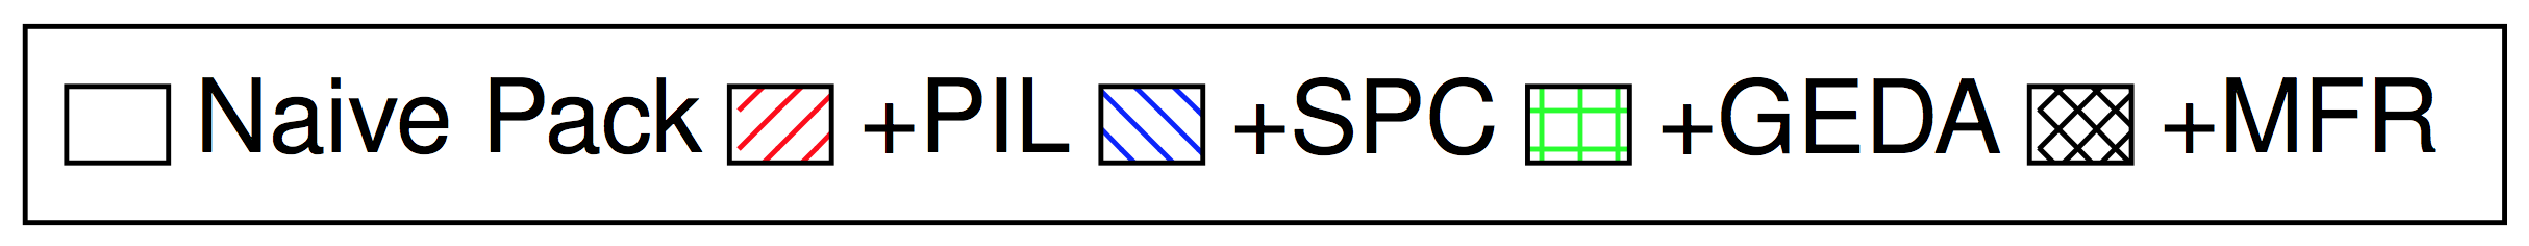
\includegraphics[width=2.5in]{F/colo/legend}
}
\centerline{

\begin{tikzpicture}[font=\sffamily\footnotesize]
\begin{axis}[
xbar stacked,
y=5mm,
width=3.1in,
xmin=0, xmax=512,
bar width=3mm,
symbolic y coords={VOLD, RIAK, CASS2, CASS1},
ytick=data,
yticklabels={{(d) Voldemort, (c) Riak, (b) Cass-2, (a) Cass-1}},
every axis y label/.style={at={(ticklabel cs:0.5)},rotate=90,anchor=near ticklabel},
axis y line*=left,
enlarge y limits={0.25},
legend style={at={(0.5,1.3)},anchor=north,legend columns=-1},
xmajorgrids=true,
xlabel=\#Nodes
]
\addplot [fill=white] plot coordinates {(80,VOLD) (16,RIAK) (48,CASS2) (48,CASS1)}; %mpc
\addplot [pattern=north east lines, pattern color=red] plot coordinates {(0,VOLD) (0,RIAK) (12,CASS2) (0,CASS1)}; %+pil
\addplot [pattern=north west lines, pattern color=blue] plot coordinates {(140,VOLD) (0,RIAK) (4,CASS2) (72,CASS1)}; %+spc
\addplot [pattern=grid, pattern color=green] plot coordinates {(0,VOLD) (0,RIAK) (448,CASS2) (16,CASS1)}; %+geda
\addplot [pattern=crosshatch, pattern color=black] plot coordinates {(292,VOLD) (48,RIAK) (0,CASS2) (0,CASS1)}; %+lma
\addplot [pattern=north east lines, pattern color=red] plot coordinates {(0,VOLD) (192,RIAK) (0,CASS2) (376,CASS1)}; %+pil
\addplot [pattern=north west lines, pattern color=blue] plot coordinates {(0,VOLD) (256,RIAK) (0,CASS2) (0,CASS1)}; %+spc
%\legend{Naive Pack,+PIL,+SPC,+GEDA,+MFR}
\end{axis}
\end{tikzpicture}

\if
Cassandra1
MPC: 48
SPC: 120 (+72)
SPC + GEDA: 136 (+16)
SPC + GEDA + PIL: 512 (+376)

Cassandra2
MPC: 48
PIL: 60 (+12)
PIL + SPC: 64 (+4)
PIL + SPC + GEDA: 512 (+448)
All: 512

Riak1
MPC: 16
LMA: 64 (+40)
LMA + PIL: 256 (+192)
SPC + LMA + PIL: 512 (+256)

Voldemort1
MPC: 80
SPC: 220 (+140)
MFR: 512 (+292)
\fi

}
\mycaption[Maximum colocation factor]{fig-colo}{Maximum colocation factor}{}


\end{figure}


\if 0
\hsg{RIAK: find the final value., 
VOLD: how to speed up experiment time?? 
still waiting for network bypass??}
\fi


% independent
Second, distributed systems are implemented in different ways.
Thus, integrations to different systems face different sequences of
bottleneck.  To show this, we tried different {\em integration sequences}.
For example, 
%for reproducing \caone 
in Cassandra (Figure \ref{fig-colo}a),
our integration sequence is: +SPC, +GEDA, and +PIL (as we continuously hit
CPU contention).
%
For Riak (Figure \ref{fig-colo}c), we began with MFR as we hit
a memory bottleneck first (the excessive Erlang processes;
\sec\ref{sc-mfr}).
%\voldone in 
For Voldemort and HDFS (Figure \ref{fig-colo}d-e), we began with SPC to
reduce Java VM memory overhead.



Third, not all features get the chance to show their benefits, as the
fundamental bottlenecks are reached.  For example, for Cassandra and HDFS
(Figures \ref{fig-colo}a-c), MFR is unnecessary as we will hit CPU
contention in $>$512 nodes.  For Riak (Figure \ref{fig-colo}c),
GEDA is not needed as we will hit a memory bottleneck in $>$512 nodes, and
similarly for Voldemort (Figure \ref{fig-colo}d).




% showing its full potential
Fourth, an \sck technique can hit a different bottleneck before showing
its full potential.  For example, for Cassandra, we tried two different
integration sequences (Figure \ref{fig-colo}a-b).  With Naive Packing
(\sec\ref{sc-np}), we initially hit a MaxCF of 48 nodes due to CPU
contention.  At this point, there are two choices: add SPC+GEDA (to reduce
process/thread context switching) or PIL (to reduce expensive processing).
In Figure \ref{fig-colo}b, we tried +PIL first and we found that it does
not help much as process/thread queuing delays are still the bottleneck.
Similarly, in Figure \ref{fig-colo}a, SPC+GEDA also can only reach a
certain maximum.  This again highlights that it is the {\em combination}
of the techniques that make \sck powerful.





% ----------------------------------------
\subsection{Putting It All Together}
\label{sc-summ}





\ni {\bf Integration steps:} We now summarize how our four \sck techniques
can be integrated to a target system.  

% All the steps below are performed
% on one machine, except step \#3.

{\bf (1)} We first reduce memory footprints with SPC (\sec\ref{sc-spc})
and MFR (\sec\ref{sc-mem}) to avoid out-of-memory exceptions.  
We then modify the target system with GEDA (\sec\ref{sc-geda}) to
remove excessive thread context switching.  

{\bf (2)} Next, before running \sck with PIL, we must find all
PIL-replaceable functions (\sec\ref{sc-pil-1}, \sec\ref{sc-pil-2}) and
interpose them to record the inputs, outputs, processing time, and
non-deterministic events (\sec\ref{sc-pil-3}, \sec\ref{sc-pil-4}).

%{\bf (3a)} After the preparation, we execute the pre-memoization step in a
%real deployment.  For example, if a customer reports a problem in a
%500-node deployment, the developers should record pre-memoization data and
%profiling time from a 500-machine deployment.  Note that this step is only
%executed one time.
%
%{\bf (3b)} However, if the target protocol has non-pertinent outputs, we
%can perform time profiling with input sampling on one machine
%(\sec\ref{sc-pil-4}).

{\bf (3a)} After the preparation, if the target protocol exhibits
non-pertinent outputs, we can simply perform offline time profiling without
pre-memoization (\sec\ref{sc-pil-4}).

{\bf (3b)} Otherwise, we execute the pre-memoization step
(\sec\ref{sc-pil-3}).  For example,
%if a scalability problem is reported in an $N$-node deployment, 
if we want to scale-check an $N$-node deployment, 
we record pre-memoized data and in-situ profiled time with
colocation factor of $N$.  

{\bf (4)} Finally, we begin scale-checking the target protocol with all
the features enabled, including PIL.  This scale-check phase will use the
recorded output and time profiles and run in deterministic order.

Note that all these features are only enabled in \sck mode.  In online
deployment, the system runs normally as if without any changes and
modification overhead.


\vni {\bf Debugging efficiency:} We now emphasize how \sck eases
scale-checking and large-scale debugging efforts.  

First, the only step that consumes time is the time
profiling and pre-memoization phase (step 3).\footnote{Ranges
1-34 hours for 100-500 nodes.}  This is because nodes
compete for CPU resources (PIL is still disabled).  However, this is only
a {\em one-time} overhead.
%

Second and most importantly, developers can {\em repeatedly re-run} the
scale-check phase (step 4) as many times as needed (tens/hundreds of
iterations) until the bug's root cause is found.  In this phase, the
target protocol runs in a {\em similar} duration and behavior as if all
the nodes run on independent machines.

%
Finally, developers can quickly apply and test new fixes.
%
Some fixes can be tested by only re-running the last phase; for example,
fixes such as
%
changing the failure detector \phi threshold (for \caone),
%
caching slow methods (\catwo),
%
changing lock management (\cafour), and
%
enabling parallel processing (\voldone).
%
% In our evaluation, we have applied all the above fixes in \sck and
% observed the patch results.
%
However, if the fixes involve a complete redesign (\eg, optimized gossip
processing in \catri, decentralized to centralized rebalancing in
\riakone), the integration and profiling/pre-memoization steps (2 and 3)
must be repeated.









\if 0

For riak1, developers re-design the bootstrap process.  Previously, it was
p2p process, that everyone helped gossiping the partition table.  But in
the new version, the developers changed the process.  Now, we ask one node
to be a centralized node calculating final partition table and gossip it
to every node.

For cass3, developers optimized the slow method, remove unnecessary
computation.  So the execution time will be different.

Here are the bugs that don't need new order determinism

In cass1, developers did not change how message gets processed, but
changed the failure detector to be more robust for significantly long
message processing time.

In cass2, there were 2 fixes, caching the result of slow method, and make
slow method faster.  If the fix is only caching the result, we can apply
it directly to suck phase.  But the second fix needs to run order
determinism again.

In cass4, previously, Cassandra acquires a lock and then processes, and it
acquires the lock for long time, so it blocks other executions.  The fix
is Cassandra will acquire the lock and then make a copy of necessary data
structure then processes on the copy. The processing was not changed.

I think in general fixes that can be tested without new order determinism are

- configuration change

- change the way we call problematic methods (e.g. releasing lock before
processing, decrease the number of method call).


\fi

\if 0
riak: 11690 -- 6800 seconds.
cass1: 15 minutes -- 1.5 minutes.
cass2: ??? never wait .. 
cass3: 
cass4: 
\fi


\fi

We now present \sck, a ``scale-check'' approach that helps
developers find and reproduce real-scale scalability bugs on one machine.
%
From our bug study, we find that the major root cause of scalability bugs
is {\em scale-dependent loops} (\eg, a \oonnn loop that iterates through
scale-dependent data structures such as lists of node descriptors).
%
Thus, the goal of \sck is to find and test such loops and reveal their
potential bug symptoms accurately.
%
To achieve this, \sck address the three challenges below.


%  sfind
First, {\em how to find ``hidden'' scale-dependent loops?}  Such loops can 
span across multiple functions and iterate a variety data structures; in
Cassandra, \oonnn loops span 1000+ LOC across 3 classes and 10 functions
and iterate three different scale-dependent data structures.
%
To address this, we build \sfind, a static analysis tool that shows code
paths to potential scalability bugs.  With the output of \sfind,
developers can setup the necessary workload (\eg, bootstrap,
add/decommission nodes) that will exercise the potentially buggy paths.

% stest
Second, {\em how to create a one-machine scalable test framework?}  One 
important finding we made is that current distributed systems are not 
built with single-machine scale-checkability in mind.  Naively packing
nodes on one machine quickly hits a colocation limitation
($<$100 nodes).  Thus, we build \stest, a scalable testing approach that
contains a series of colocation techniques such as running nodes as a
single process and removing unnecessary memory allocations.  Furthermore,
to reduce context-switching delays of hundreds/thousands of threads
in \stest, we restructure the target systems into a global event driven
architecture (GEDA), a derivative of SEDA \cite{Welsh+01-Seda}, where
stages, queues, and worker threads are shared by the whole cluster.

% stest-mem
Finally, {\em how to produce accurate results (bug symptoms)?}  One major
challenge of \sck is how to colocate hundreds of CPU-intensive nodes on
one machine, but still achieve high accuracy (\ie, observe a similar
behavior as in the real-scale deployment).
%
We introduce {\em processing illusion} (PIL), an emulation technique that
replaces scale-dependent CPU-intensive computations with \sleep, without
changing the cluster behavior.  The insight behind PIL is that the key to
computation is not the intermediate results, but rather the execution time
and eventual output.  \sck automatically finds PIL-replaceable functions,
inserts pre-memoization code that records the input-output-time pairs in
the first test run, replaces them with \sleep, and replays the code
deterministically in subsequent replay runs.


% ------------
To show the generality of \sck, we have integrated \sck to
Cassandra \cite{Lakshman+09-Cassandra}, HDFS \cite{HDFSWeb},
Riak \cite{RiakWeb}, and Voldemort \cite{VoldemortWeb},
across a total of  \numVersTotal old and new releases.
%
We scale-checked a total of \numProt protocols (bootstrap, rebalance,
add/decommission nodes, \etc), reproduced \numEval old
and found 2 new scalability bugs.
%
\sck can achieve a colocation
factor of around 500 nodes on a 16-core machine with high result accuracy.


\subsection{\sfind}
\label{sc-find}

Manually finding scale-dependent loops is not trivial.  Such loops can
span across multiple functions and iterate on different scale-dependent data
structures.  In Figure \ref{fig-code}, The \oonnn loops span 1000+ LOC
across 3 classes and 10 functions.
%
This difficulty motivates \sfind, a generic program analysis that helps
developers pinpoint scale-dependent loops.  The following subsections
discuss the three main steps in \sfind.







\begin{figure}[t]

\centerline{
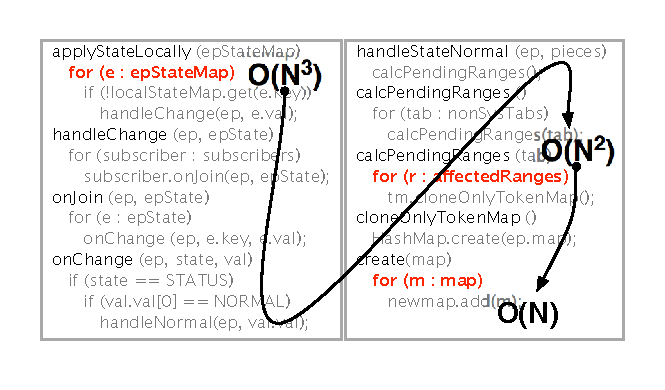
\includegraphics[height=1.7in]{F/ill/code1.eps}
%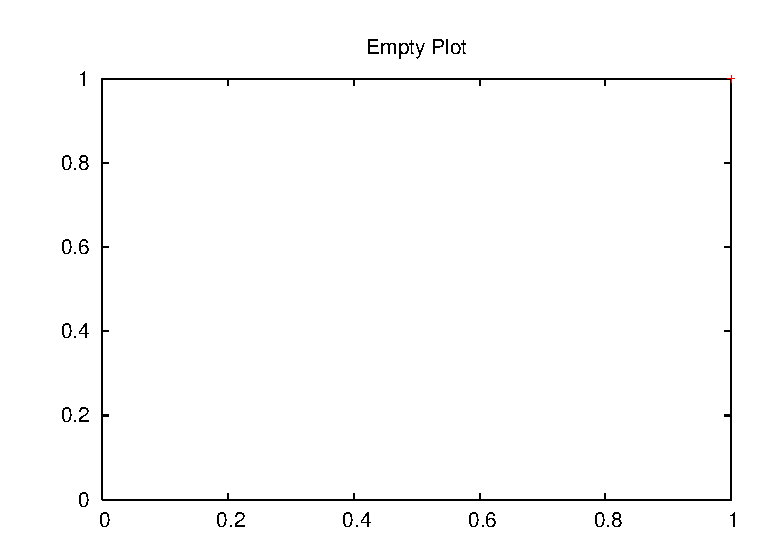
\includegraphics[height=0.6in]{F/empty.eps}
}
\vminten
\mycaption{fig-code}{\oonnn scale-depended loops}{The partial
code segment above details the \oonnn loop
in Figure \ref{fig-mot}.
Note that not all loops are scale-dependent loops.
The \ts{epStateMap}, \ts{affectedRanges}, and \ts{map}
variables are not the annotated scale-dependent variables, 
however \sfind taints them with a dataflow analysis.
}
\vminfive
\end{figure}



% $O(n^3)$ loop spans 6 functions with 188 LOC in between each pair of loops.


% ------------------------
\vni {\bf (1) Annotating scale-dependent data structures:} To use \sfind,
developers first lightly annotate scale-dependent data structures (whose
size increase as the cluster size grows).
%
For example, related to \caone (Figure \ref{fig-code}), we annotate seven
data structures and \sfind automatically taints other variables that point
to the same structures (\eg, \ts{epStateMap}, \ts{affectedRanges}, and
\ts{map} in Figure \ref{fig-code} are pointers to the annotated data
structures).


%(\ts{endpointStateMap}, \ts{tokenToEndpointMap},
%\ts{endpointToHostIdMap}, and \ts{bootstrapTokens});



% ------------------------
\vni {\bf (2) Finding scale-dependent loops:}
%
With the annotations, \sfind can then automatically find scale-dependent
loops with the following steps:
%
(a) perform a data-flow analysis to taint other pointers derived from the
original scale-dependent variables,
%
(b) taint loops (\ts{for}, \ts{while}) that iterate through the variables,
%
(c) perform a control-flow analysis to construct the nested Big $O$
complexity of each loop,
%
(d) identify the nested-loop contents (CPU/instructions only, IOs, or
locks).
%
With these steps, in Figure \ref{fig-code} for example, \sfind can mark
\ts{applyStateLocally} as an \oonnn function.


We also notice a special case of 
scale-dependent ``loops'': 
In master-worker architecture, a synchronized master's function
that is being called by all the worker nodes implicitly forms a ``loop''
(examples in \sec\ref{eval-bugs}).  
%
\sfind also handles such a scenario; the developers simply annotate the
master RPC class and \sfind automatically searches for locking
functions called by the worker nodes.  \sfind also differentiates
functions that are called within the client read/write paths (higher call
frequency) and by background periodic threads.

% if have space:
%
% Developers can prioritize those within the
% client paths, as they run most of the time.
%
% Due to space constraints, we omit discussion of other challenges such as
% abstract classes, \xxx

% ------------------------
\vni {\bf (3) Reporting and triaging:}
%
Before producing a report, \sfind performs a simple triaging.  For
example, if a function $g$ has a lower complexity than $f$ and $g$ is
within the call path of $f$, then developers can prioritize testing $f$.
%
For every nested loop to test, \sfind reports the relevant control- and
data-flows from the outer-most to inner-most loop, along with the entry
points (either client/admin RPCs or background daemon threads).
%
This helps developers create the necessary test workloads.  For example,
in Figure \ref{fig-code}, the \oonnn path is only exercised if the cluster
bootstraps from scratch; peers do not know about each other (hinted from
the \ts{if(!localStateMap.get())}, \ts{onChange()}, \ts{state==STATUS} and
\ts{val==NORMAL}).

% creating the unit tests
We note that creating test workloads from \sfind's reports is a manual
process.  Automated test generation is possible for single-machine
programs/libraries \cite{Cadar+08-KLEE}, however we are not aware of any
work that automates such process in the context of real-world, complex,
large-scale distributed systems.
%
We put our work in the context of DevOps culture
\cite{Limoncelli+11-Devops} where developers are testers and testers are
developers, which simplify testing efforts.



\if 0
With this triaging, we reduce the
number of tests.  For example, in Cassandra, out of 22 \oonn and 9 \oonnn
functions, they are accessible by 3 \oonnn functions.
\fi


% the content of the loop
% (CPU, lock, IO) along with the total number of LOC inside the loop, which
% can help developers to prioritize.




\subsection{\stest}
\label{sc-test}


% if no space, change subsection into just 

The next challenge to address is: can we test hundreds of nodes on one
machine?  To achieve a scalable testing framework with a high colocation
factor (\eg, 500 nodes), we have to make a series of collocation
engineering efforts.  Below we describe and name them (with abbreviations)
for ease of reference in the evaluation.

% ----------------------------------------
\subsubsection{Naive Packing (NP)}
\label{sc-np}

The easiest setup to test scale-dependent loops is to (naively) pack all
the nodes as processes on a single machine.  However, with 32 GB DRAM, we
can only reach  a colocation factor of 50 (far from the desired target),
which is caused by two reasons.

First, many distributed systems today are implemented in managed languages
(\eg, Java, Erlang) whose runtimes consumes non-negligible memory overhead.
Java and Erlang VMs for example use around 70 and 64 MB of memory per
process respectively.  A high colocation factor is not attainable.
%
We also tried running nodes as Linux KVM VMs and using KSM (kernel
samepage merging) tool.  Interestingly, the tool does not find many
duplicate pages even though the VMs/processes are similar.  We leave further
investigation for future work.

Second, a managed-language VM is backed by advanced services.  For
example, Erlang VMM contains a DNS service that sends heartbeat messages
among connected VMs.  As hundreds of Erlang VMs (one for each Riak node)
run on one Erlang VMM, the heartbeat messages cause a ``network'' overflow
that undesirably disconnects Erlang VMs.


% ----------------------------------------
\subsubsection{Single-Process Cluster (SPC)}
\label{sc-spc}

To address the bottlenecks above, we run all nodes as threads in a single
process.  Surprisingly, some parts of our target systems are not easy to
run in this ``single-process cluster'' mode.  Thus, we need to slightly
re-design our target systems (\eg, putting global variables modularly into
classes, adding arrays of global node descriptors, removing
static-synchronized functions that lock the whole cluster).



% ----------------------------------------
\subsubsection{Memory Footprint Reduction (MFR)}
\label{sc-mfr}

While SPC reduces the memory footprints of the language runtime, in some
target systems, we are still hit with out-of-memory exceptions, coming
from system-specific high memory usage, as in the examples below.

First, some protocols can ``over-allocate'' memory unnecessarily.
%
For instance, in Riak's rebalance protocol, each node creates
$N$$\times$$P$ partition services although at the end only retain $P$
partitions and remove the other $(N$$-$$1)$$\times$$P$ services (as
rebalanced to other nodes).
%
Each partition service is an Erlang process (1.3 MB of memory overhead);
colocating 30 nodes ($N$$=$30 with the default $P$$=$64) will directly
consume 75 GB of memory (30$\times$30$\times$64$\times$1.3 MB) from the
start.
%
We must manually modify Riak to remove this unoptimized memory usage.


Second, some libraries can cause high memory footprints.  For example,
Voldemort nodes use Java NIO \cite{VoldemortNIO} which is fast but
contains buffers and connection metadata that take up memory space.
%
To address this, we leverage the fact that in SPC, all nodes run in one
process, hence user-kernel/library switching to send messages becomes
unnecessary.  Thus, we create a shim layer in our target systems to bypass
OS/library network calls when they run in \stest mode.




% First, the ``\ts{main()}'' function of each node creates many services
% and global data structures (system metadata) that are never used by the
% target protocol.  For example, in Cassandra, \ts{Migration},
% \ts{Storage}, and \ts{Compaction} services are memory intensive but not
% needed for scale-checking the bootstrap protocol, which only needs the
% \ts{Gossip} and \ts{FailDetector} services.  In \sck, services are
% lazily called (not created until used).


% ----------------------------------------
\subsubsection{Global Event Driven Arch. (GEDA)}
\label{sc-geda}

% if have space, show GEDA architecture

After applying SPC and MFR, we faced another challenge.  As each node
still runs multiple daemon threads (gossiper, failure detector, \etc), a
high colocation factor will spawn more than one thousand threads, which
causes two problems.  First, the OS/runtime limits the number of native
threads per-process (which can be modified), but second, the problem
causes severe context switching and queuing delays; we noticed that
events become late (\eg, gossips are not sent every second).


To address this, we leverage the staged event-driven architecture (SEDA)
\cite{Welsh+01-Seda} common in distributed system implementations.  With
SEDA, each service/stage in each node exclusively has an event queue and a
handler thread.  In \stest mode, we convert SEDA to {\em global-event
  driven architecture} (GEDA).  That is, for every stage, there is only
{\em one} queue and one/few handlers for the {\em whole} cluster.

As an example, let's consider a periodic gossip service.  With 500-node
colocation, there are 500 threads in SPC, each sending a gossip every
second.  With GEDA, we only deploy a few threads (matched with the number
of available cores).  These global handler threads are shared among all
the nodes for sending gossips.  As another example, for gossip processing,
there is only one global gossip-receiving queue shared among all nodes.
%
Overall, GEDA removes some delays that should have never existed in the
first place, as if the nodes run exclusively on independent machines.
GEDA does not change the logic of the target systems.


% Riak
We interestingly found that in Erlang-based Riak, SPC is sufficient (no
thread context-switching delays).
This is because Erlang is an event-driven language.
%
Upon program start-up, Erlang (implicitly) starts a
scheduler process per core.
%
When ``Erlang processes'' (threads) run, their
events are automatically scheduled; 
for example, when an Erlang process $X$ sends a message to $Y$,
the message is automatically put to a runtime queue and scheduled.
%
Thus, Erlang processes behave like event handlers, while the
scheduler processes are synonymous to GEDA threads.
%
An event-driven programming framework can ease \sck, but
still SPC and MFR are needed.


% -------------------------------------------------
\subsubsection{Lessons Learned}


From this experience, we make a conclusion that existing distributed
systems are not built with (single-machine) scale-checkability in mind.
There were no direct utilities to be used for solving a variety of
colocation bottlenecks above.  Our colocation techniques above
collectively create a viable solution to make distributed systems
single-machine scale-checkable.  





\subsection{Processing Illusion (PIL)}
\label{sc-pil}

While I/O and memory bottlenecks are often blamed for many scalability problems
\cite{Ousterhout+15-MakingSense,Konstantin+10-HDFSScalability, Wang+14-Exalt},
scalability bugs also could be caused by cascading impacts of CPU-intensive
processing as the example of Cassandra bugs.
%
To emulate CPU-intensive processing, we introduce {\em processing illusion}
(PIL), an approach that {\em replaces an actual processing with \sleep}.  For
example, in the sample Cassandra bug, we can replace the expensive ring-table
update with \ts{sleep(t)} where \ts{t} is an accurate timing of how long the
update takes.


The intuition behind PIL is similar to the intuition behind other
emulation techniques.
%
For example, Exalt provides an illusion of storage space; their insight
was ``how data is processed is  not affected by the content of the data
being written, but only by its size'' \cite{Wang+14-Exalt}.
%
PIL provides an illusion of compute processing; our insight is that
{\em ``the
  key to computation is not the intermediate results, but rather the
  execution time and eventual output''.}
% {\em ``how
%   compute matters is not because of the intermediate computation, but 
% rather by its execution time and output.''}
%

PIL might sound outrageous in the first place, but it is feasible only if 
the following concerns are addressed:
%
% replace compute with sleep
%
How can a function be safely replaced with \sleep \textit{without} changing the
whole processing semantic?  And how to find specific functions that should be
replaced with \sleep?
%
How can we produce the output if the actual compute is skipped?
%
How can we predict the actual compute time (\ts{t}) accurately?

\subsubsection{PIL-Safe Functions}
\label{sc-pil-1}

Our first challenge is to ensure that functions (or code blocks) can be safely
replaced with \sleep, but still retain the cluster-wide behavior and unearth the
bug symptoms.  We name such functions as {\em PIL-safe functions}.
%
We identify two main characteristics of sleep-safe functions:
% by memoization
\begin{enumerate}
\item Memoizable output: a PIL-safe function must have a memoizable
(deterministic) output based on the input of the function.
% ...
\item Non-pertinent I/Os: if a function performs disk/network I/Os that are not
pertinent to the correctness of the corresponding protocol, the function is
PIL-safe.  For example, in the sample Cassandra bugs, there is a ring-table
checkpoint (not shown) needed for fault tolerance but is irrelevant (never read)
during bootstrapping.
%
\end{enumerate}
%We extend \sfind to \sfindp, which includes a static analysis that finds code
%blocks in scale-dependent loops that can be safely PIL-ed.
Depending on the modularity of the target system, manually finding such target
functions can be challenging, primarily because scale-dependent nested loops can
span across multiple functions. Right now, we rely on developers to identify
such that functions, and we leave automatic PIL-taking function extracting for
future work (Chapter \ref{chp-con}).

% -----------------------------------
\subsubsection{Pre-Memoization with Order Determinism}
\label{sc-pil-3}

As sleep-safe functions no longer perform the actual computation, the next
question to address is: how do we manufacture the output?  We find there
are sleep-safe functions with non-pertinent outputs
(\sec\ref{sc-pil-1}). For these functions, only time profiling is needed
(\sec\ref{sc-pil-4}) but not output recording.  However, there are also
sleep-safe functions with non-pertinent intermediate data but with outputs
that are needed.
%
For this latter case, we need to manufacture the outputs such that the
global behavior is not altered (\eg, cluster bootstrapping or rebalancing
should terminate successfully).
%
Our solution is {\em pre-memoization}: given a sleep-safe
function, we identify all the possible inputs, and for every input, run
the function and pre-memoize the output.  
% This is done prior to \sck; 
When \sck runs, it will use the pre-memoized outputs.


Unfortunately, pre-memoization in the context of large-scale,
decentralized, non-deterministic distributed systems requires an {\em
  ``infinite''} time and storage space.  The issue is that the state of
each node (the input) depends on the {\em order} in which messages arrive
(which can be random).
%
As an example, let's consider Riak's bootstrap+rebalance protocol where
eventually all nodes own a similar number of partitions.  
% The decentralized algorithm is quite complex \cite{algorithmOnline}, but
% put simply, each node
A node initially has an unbalanced partition table, receives another
partition table from a peer node, then inputs it to a rebalance function,
and finally sends the output to a {\em random} node via gossiping.  {\em
  Every} node repeats the same process until the cluster is balanced.
%
In a Riak cluster
with $N$$=$256 and 
$P$\footnote{$P$: the number of key-partitions per node;  
A key-partition is typically a random integer 
within 2$^{64}$ keyrange.}$=$64, there are in total 2489 rebalance iterations
with a set of specific inputs in {\em one} run.  
{\em Another} run of the protocol will
result in a {\em different} set of inputs due to gossip randomness.
%, due to the gossip randomness.
Our calculation shows that there are 
$(N^{NP})^2$ 
possible inputs.
% ; with 550-KB
% partition table, this pre-memoization requires \xxx Exabytes of space.




To address this problem, we pre-memoize with {\em order determinism}.
Thus, repeated runs of the same workload in \sck mode will use the {\em
  same} global message ordering (akin to deterministic record and replay
\cite{Geels+07-Friday}).
% Gautam+09-ODR,   Geels+06-Liblog, Guo+08-R2, Soyeon+09-PRES
%
For example, across different runs, a Riak node now receives gossips from
the same sequence of nodes.
%
With order determinism, pre-memoization and \sck work as follow: 
%
% {\bf (1)} We first run the whole cluster on a real deployment and interpose
% sleep-safe functions.
\begin{enumerate}
\item We run all nodes on one machine
without PIL (more details in \sec\ref{sc-summ}) and interpose
sleep-safe functions.
%
\item When sleep-safe functions are executed, we record the inputs and
corresponding outputs to a {\em memoization database} (SSD-backed files).
%
\item During this pre-memoization phase, 
we {\em record message non-determinism} (\eg,
gossip send-receive pairs and their orderings).
%
\item After pre-memoization completes, we can 
repeatedly run \sck wherein order
determinism is enforced (\eg, no randomness), sleep-safe functions
replaced with PIL, and their outputs retrieved from the memoization
database.
%
%Note that steps 1-3 are the only steps that require real deployment.  
\end{enumerate}
We omit some details above but will summarize the steps again later along
with other features (\sec\ref{sc-summ}).


%
With order determinism, the memoization database is kept small as we only
record the possible inputs within {\em one} deterministic order.  In the
256-node Riak's case above, the database only needs to store around 2500
input-output pairs (the number of rebalance iterations observed) in 1.3 GB
of memoized data (and 5.3 GB for the 512-node setup).
% remove if no space
We also note that while the idea of deterministic systems has been made
popular recently,
% \cite{Aviram+10-Determinator, Bergan+10-dOS}, 
the concept of deterministic distributed systems is still not practical
due to the excessive runtime overhead (\eg, 10x slower
\cite{Hunt+13-DDOS}).  However, in the context of offline methodology such
as \sck, order determinism can be exploited in a fitting manner.




% -----------------------------------
\subsubsection{Time Profiling}
\label{sc-pil-4}

As sleep-safe functions are replaced with \ts{sleep(t)}, we need to
accurately predict the actual compute time (\ts{t}).  There are two
different approaches we take, depending on the target protocols.
%
\begin{enumerate}
\item The first approach is to profile compute time in situ with
the pre-memoization phase ({\em in-situ time profiling}).  
That is, for each input observed during
pre-memoization, we also record how long the processing takes.
%
\item Another approach is to profile compute time with an {\em offline
time  profiling}, which is feasible for functions with non-pertinent outputs
(\sec\ref{sc-pil-1}), which do not need pre-memoized outputs.  
\end{enumerate}

With offline time profiling, we simply profile the expensive function
exclusively by itself with the possible input space.
If faster profiling is needed, we can sample the input space.
For example, in the sample Cassandra bug,
the expensive function depends on a 2-dimensional input (\#commit states
and current ring table size), each ranges from 1 to $N$.  
With $N^2$ profiles, the profiling time can
take more than 
one day without sampling when $N$ is large (\eg, 512 nodes).  When \sck
runs, given an input, we normalize \ts{t} based on the sampled profile.

% ......
We now address two further questions.  First, is time profiling necessary?
In other words, is static prediction sufficient (\eg, extrapolation based
on a \ts{for}-loop timing)?  In our case, static prediction is hard
to achieve; nested loops can span across multiple functions with many
\ts{if-else} conditions.  For example, state-update processing in
the sample Cassandra bug can range from 0.001 to 4 seconds depending on the
multi-dimensional input (\sec\ref{mot-observe}).  
%
% \hsg{why don't we prove this by saying, we did this with static prediction,
% but we got inaccurate results. TODO??}

% Hence, time profiling is needed for accuracy.

% remove if no confirmation from Cesar \hsg{Cesar??} 

% Furthermore, processing time depends on CPU speed and storage latency.
% We observed a case of a customer deploying Riak in ``weak'' machines,
% which surfaces a scalability bug that the developers did not expect
% \cite{riak?}.  Thus, dynamic profiling time must be based on a similar
% machine deployed by the customer who reported the bugs.



% predict scalability bugs from profiling
Second, is it obvious from the profiled time that a scalability bug will
appear, hence obviating the need for \sck?  
%
As suggested earlier, every implementation is unique
(\sec\ref{mot-observe}).  In the sample Cassandra bug for example, {\em if} Cassandra
processes gossips in a multi-threaded manner, long processing time would
not lead to the scalability bug.
%
In fact, patches for scalability bugs do not always remove the expensive
computation.
%
Scalability bugs are not merely about the expensive functions, but rather
their potential cascading impacts, hence it is essential to run \sck 
in addition to time profiling.
% not extrapolation
We want to emphasize that our profiling approach is not the same as
extrapolation, which tends to stop profiling at a certain 
scale (\eg, 100 nodes)
and extrapolates the behavior for larger scales.  Our
profiling and \sck phases run at real scales.
% the same number of nodes.


\vfive Overall, PIL significantly removes processing contention and
reduces CPU utilization.  Interestingly, as we colocate more nodes, before
we hit 100\% CPU utilization, we hit other major colocation bottlenecks
such as memory exhaustion and process/thread context-switching delays.
%
For this reason, we re-architect our target systems to make them
scale-checkable with the next three optimization techniques
(\sec\ref{sc-spc}-\sec\ref{sc-mem}).



\if 0
\hsg{new:}
Exalt \cite{exalt} provides a compression technique that is powerful for
cases where storage capacity is the colocation bottleneck.
The compression technique however increases CPU utilization
and thus does not solve CPU-bottleneck colocation problem.
For example, it admits that the CPU-intensive HBase region servers
cannot benefit from Exalt colocation. 
\fi






\subsection{Putting It All Together}
\label{sc-summ}

We now summarize how all the \sck components described before
work together.


Pre-memoization and PIL complete the {\bf four
stages of \sck}, as illustrated in Figure \ref{fig-sck}a-d:
%
\textbf{\textcircled{a}} \sfind searches for scale-dependent loops
(\sec\ref{sc-find}) which helps developers create test workloads.
%
\textbf{\textcircled{b}}
%
For test workloads that show CPU busyness in all nodes, \sfindp finds
PIL-safe functions and automatically inserts our pre-memoization library
calls (\sec\ref{sc-pil}).
%
Next, \stest now works in two parts.
%
\textbf{\textcircled{c}} \stestm (without PIL) will run the test one time
to pre-memoize PIL-safe functions and store the tuples to a 
SSD-backed database file.
%
\textbf{\textcircled{d}} \stestp (with PIL) will then run by first having
\sfindp automatically remove the pre-memoization library calls, replace
the expensive PIL-safe function with \ts{sleep(t)}, and insert our code
that constructs the memoized output data.
%
\sck also records message ordering during \stestm and replays the same
order in \stestp (not shown).


\vni {\bf Benefits:} We now describe how \sck can ease real-scale
debugging efforts.
%
First, the only step that consumes  more time is the no-PIL
pre-memoization phase (Figure \ref{fig-sck}c), up to 6x longer time
than the real deployment testing (\sec\ref{eval-mem}).  
However, this is only a one-time overhead.
%This is again because nodes compete for CPU.  
%
Most importantly, developers can repeatedly re-run \stestp (Figure
\ref{fig-sck}d) as many times as needed (tens of iterations) until the
bug's negative impacts are understood.  In \stestp, the protocol under
test runs in a similar duration as if all the nodes run on independent
machines.


Second, some fixes can be applied and tried by only re-running the last
step; for example, fixes such as
%
changing the failure detector \phi threshold (for \caone),
%
caching slow methods (\catwo),
%
changing lock management (\cafour), and
%
enabling parallel processing (\voldone).
%
However, if the fixes involve a complete redesign (\eg, optimized gossip
processing in \catri, decentralized to centralized rebalancing in
\riakone), \stestm must be repeated.

